\chapter{Detalhes dos resultados}


\begin{figure}[H]
	\centering
	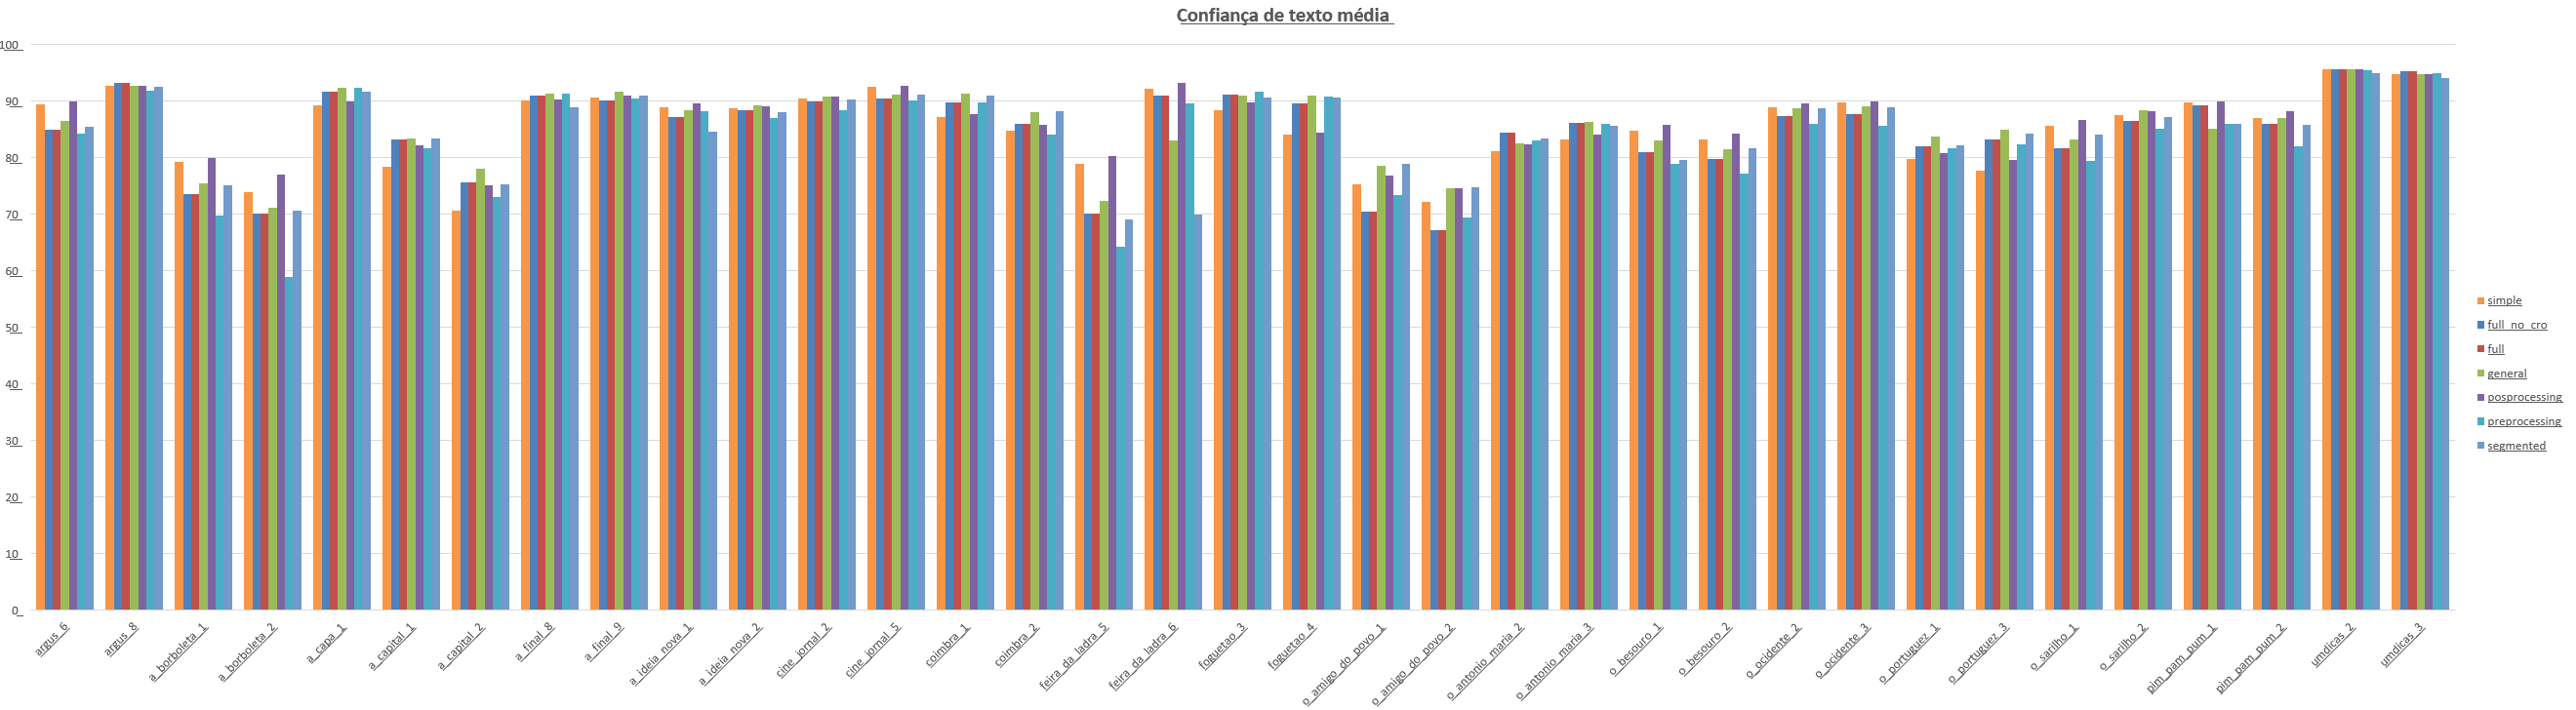
\includegraphics[angle=90,width=0.3\textwidth]{images/resultados/graph_avg_text_conf.png}
	\caption{Valores de confiança média de texto das diferentes pipelines (alargado).}
	\label{fig:graph_avg_text_conf_large}
\end{figure}



\begin{figure}[H]
	\centering
	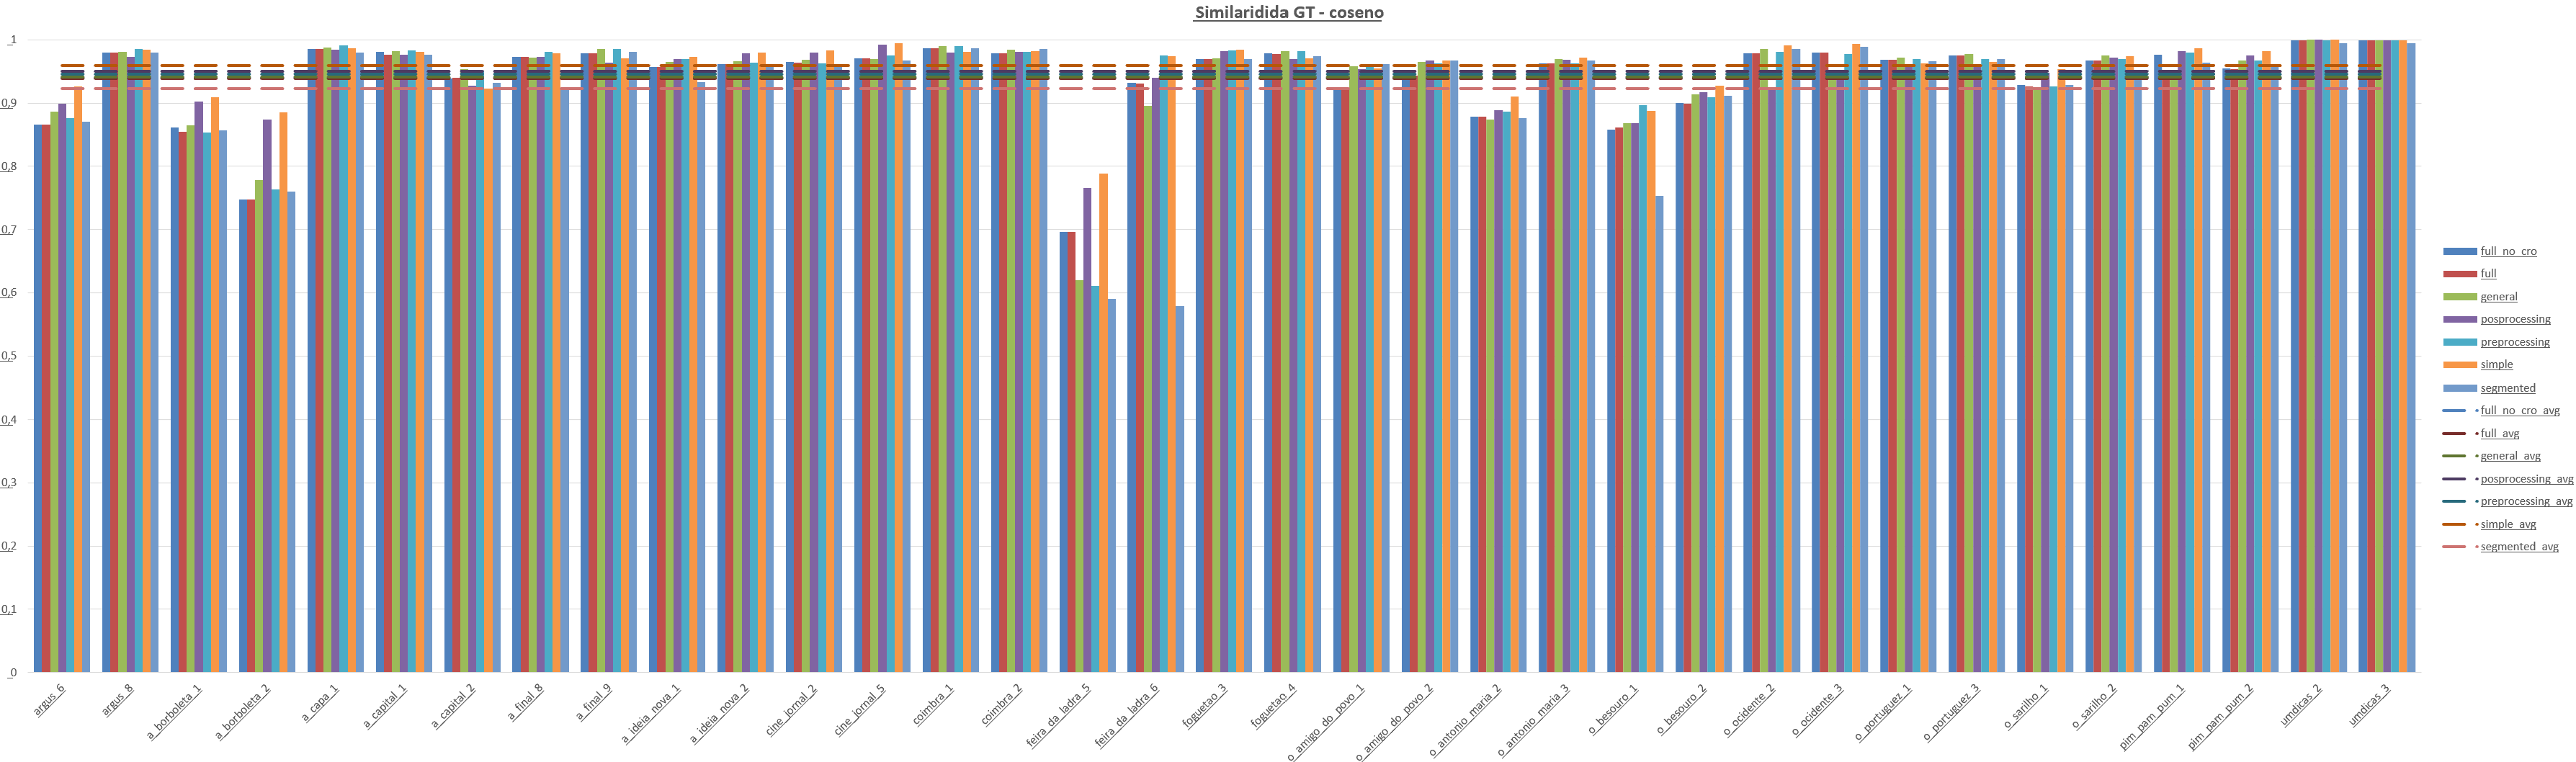
\includegraphics[angle=90,width=0.4\textwidth]{images/resultados/graph_gt_similiraty_cosine.png}
	\caption{Valores de similaridade do texto (similaridade por cosseno) com GT das diferentes pipelines (alargado).}
	\label{fig:graph_gt_similiraty_cosine_large}
\end{figure}


\begin{figure}[H]
	\centering
	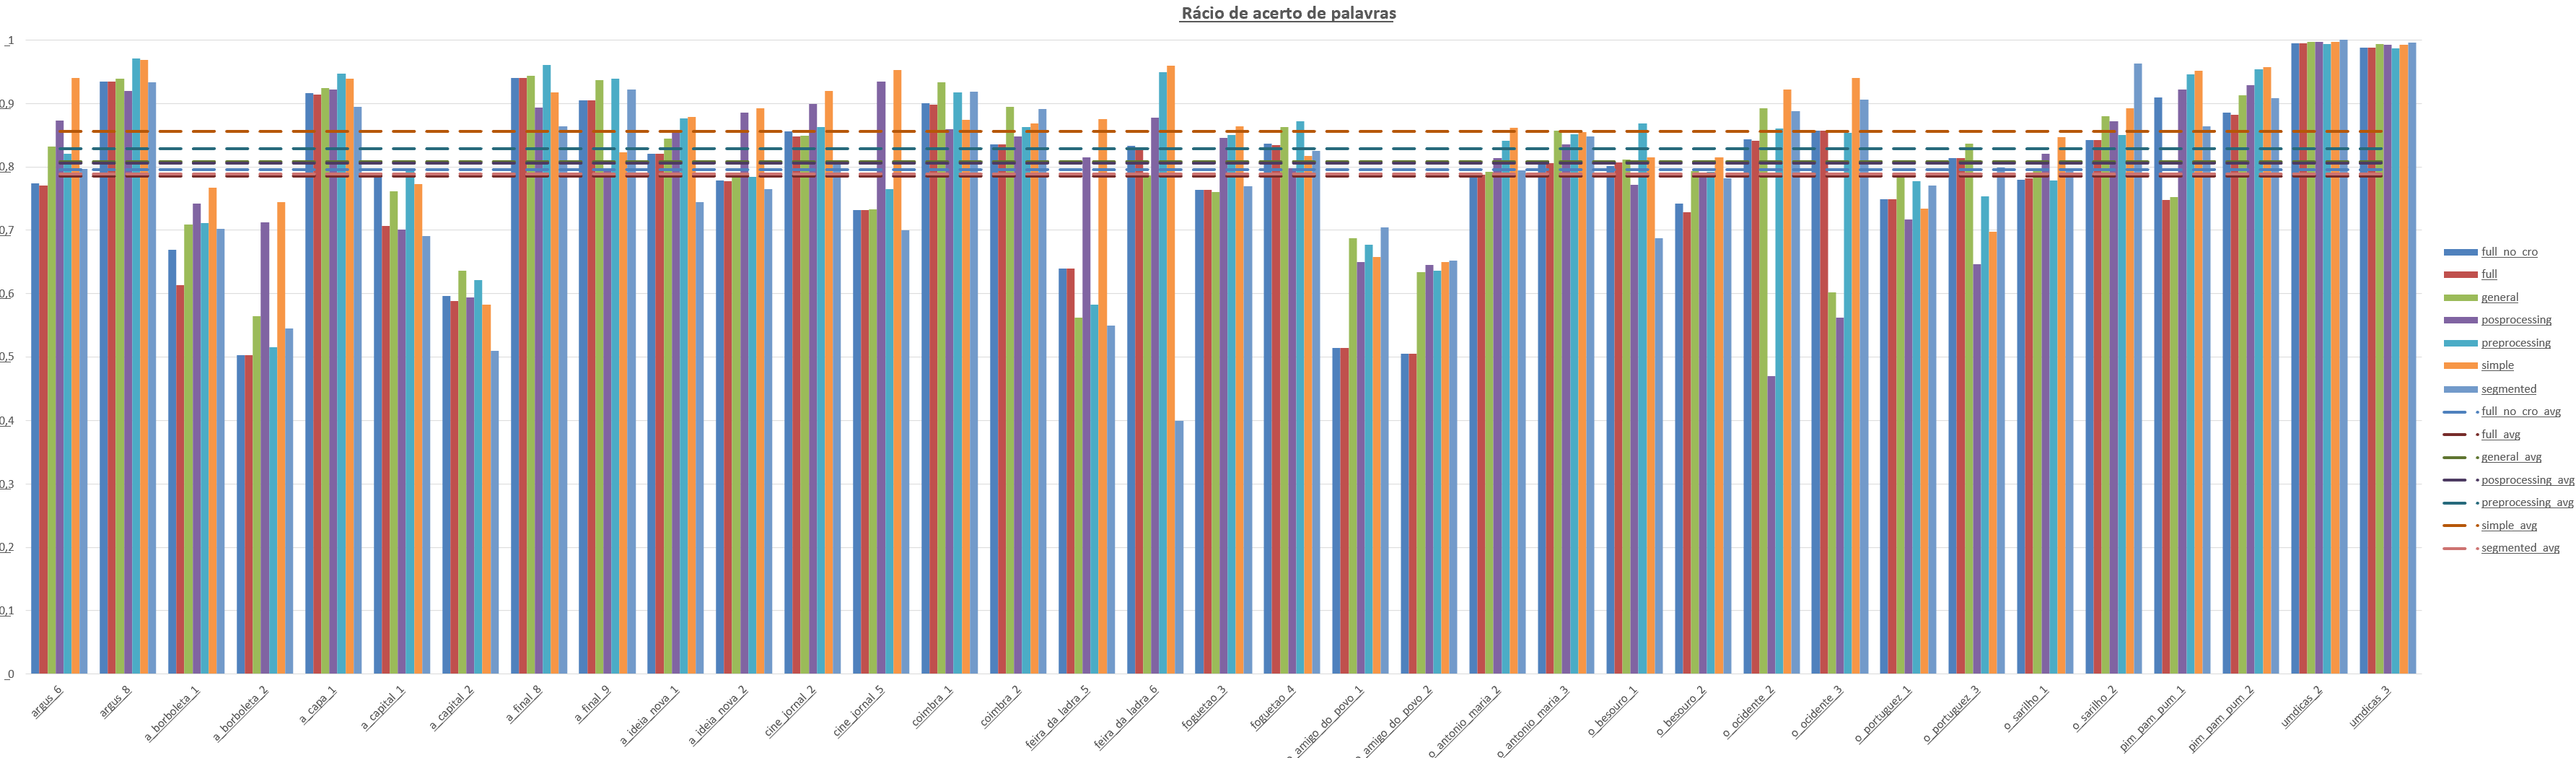
\includegraphics[angle=90,width=0.4\textwidth]{images/resultados/graph_gt_word_hit_ratio.png}
	\caption{Rácios de aparição total de palavras da GT das diferentes pipelines (alargado).}
	\label{fig:graph_gt_word_hit_ratio_large}
\end{figure}


\begin{figure}[H]
	\centering
	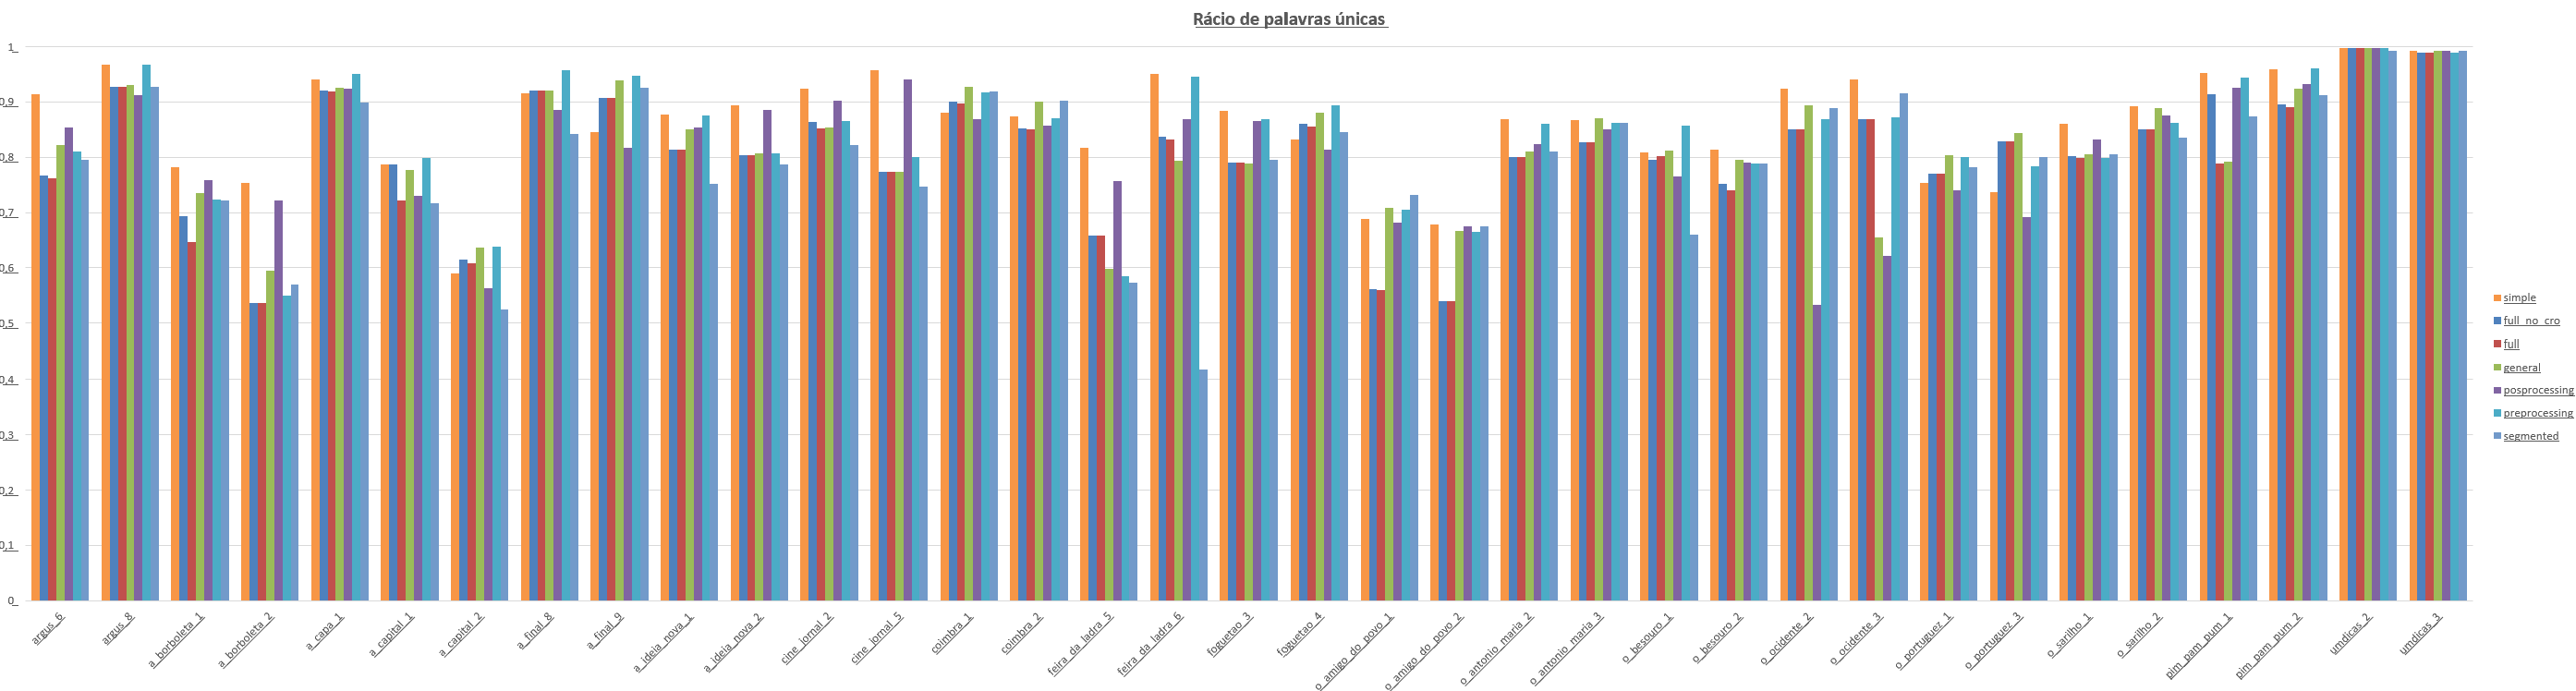
\includegraphics[angle=90,width=0.4\textwidth]{images/resultados/graph_gt_unique_word_hit_ratio.png}
	\caption{Rácios de aparição de palavras distintas da GT das diferentes pipelines (alargado).}
	\label{fig:graph_gt_unique_word_hit_ratio_large}
\end{figure}


\begin{figure}[H]
	\centering
	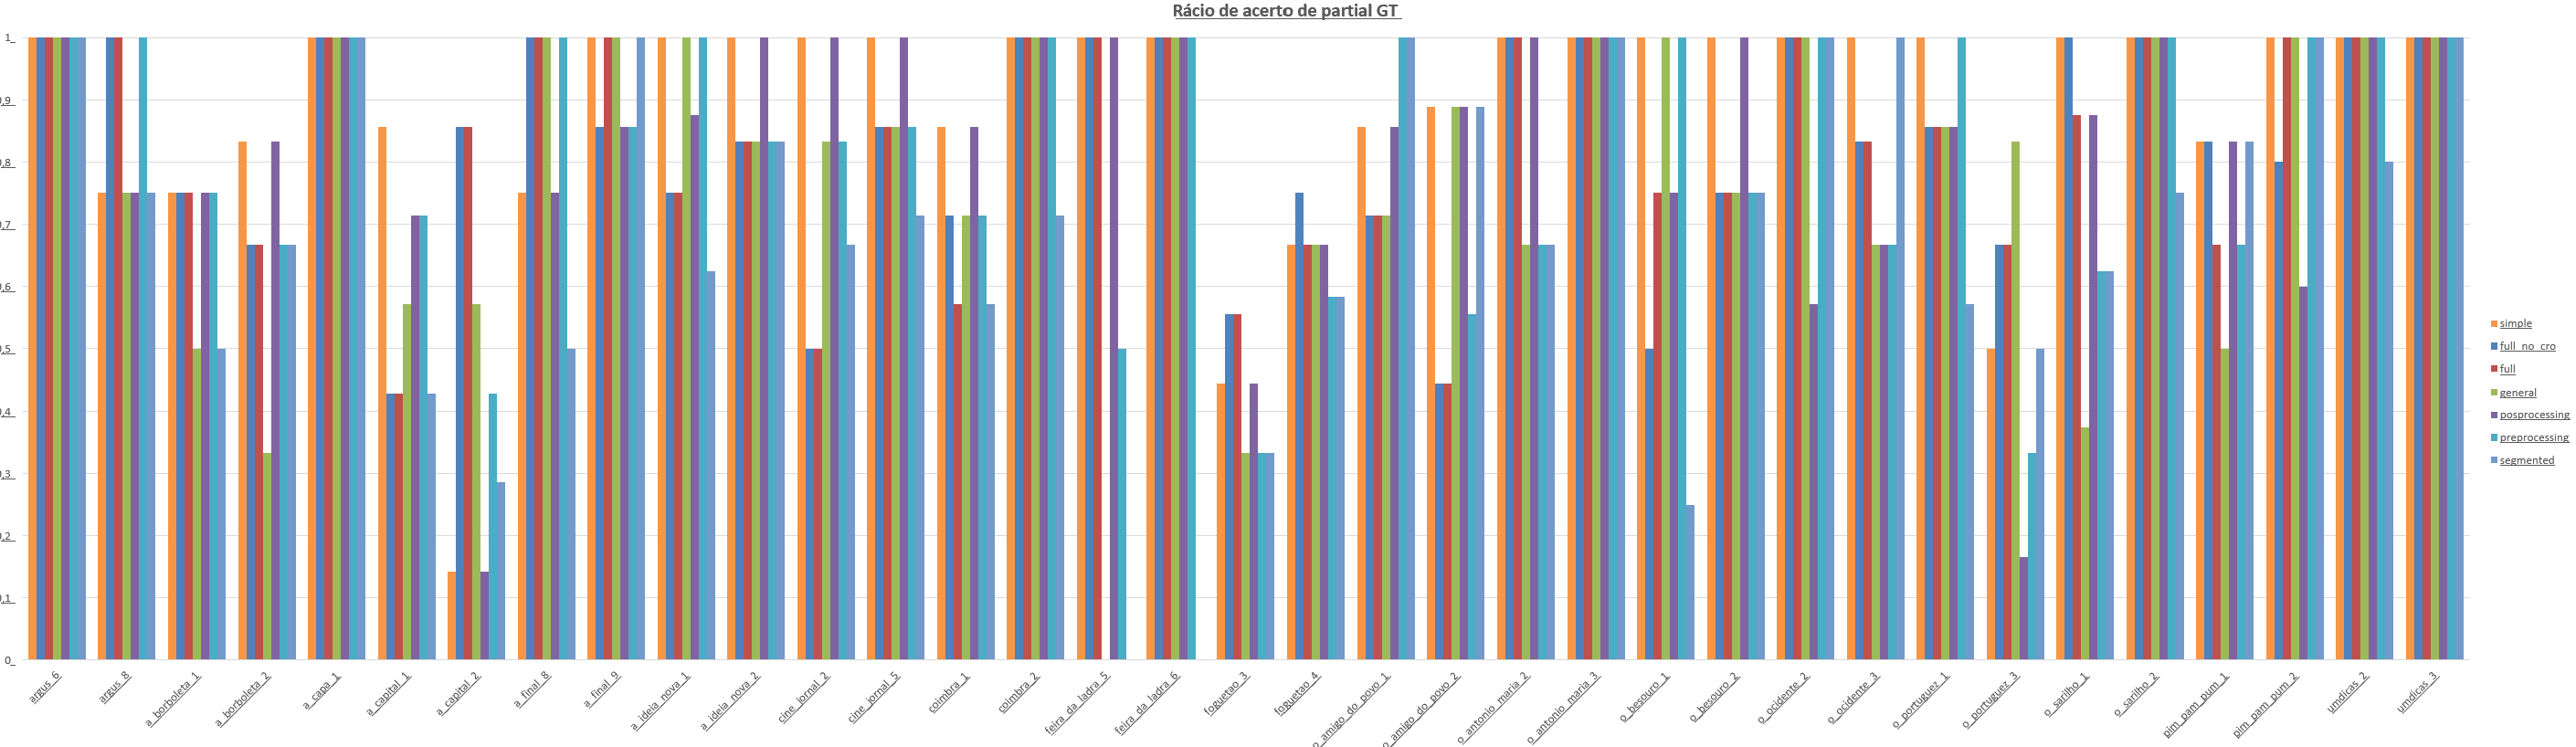
\includegraphics[angle=90,width=0.4\textwidth]{images/resultados/graph_pgt_hit_ratio.png}
	\caption{Rácios de aparição de linhas da Partial GT das diferentes pipelines (alargado).}
	\label{fig:graph_pgt_hit_ratio_large}
\end{figure}


\begin{figure}[H]
	\centering
	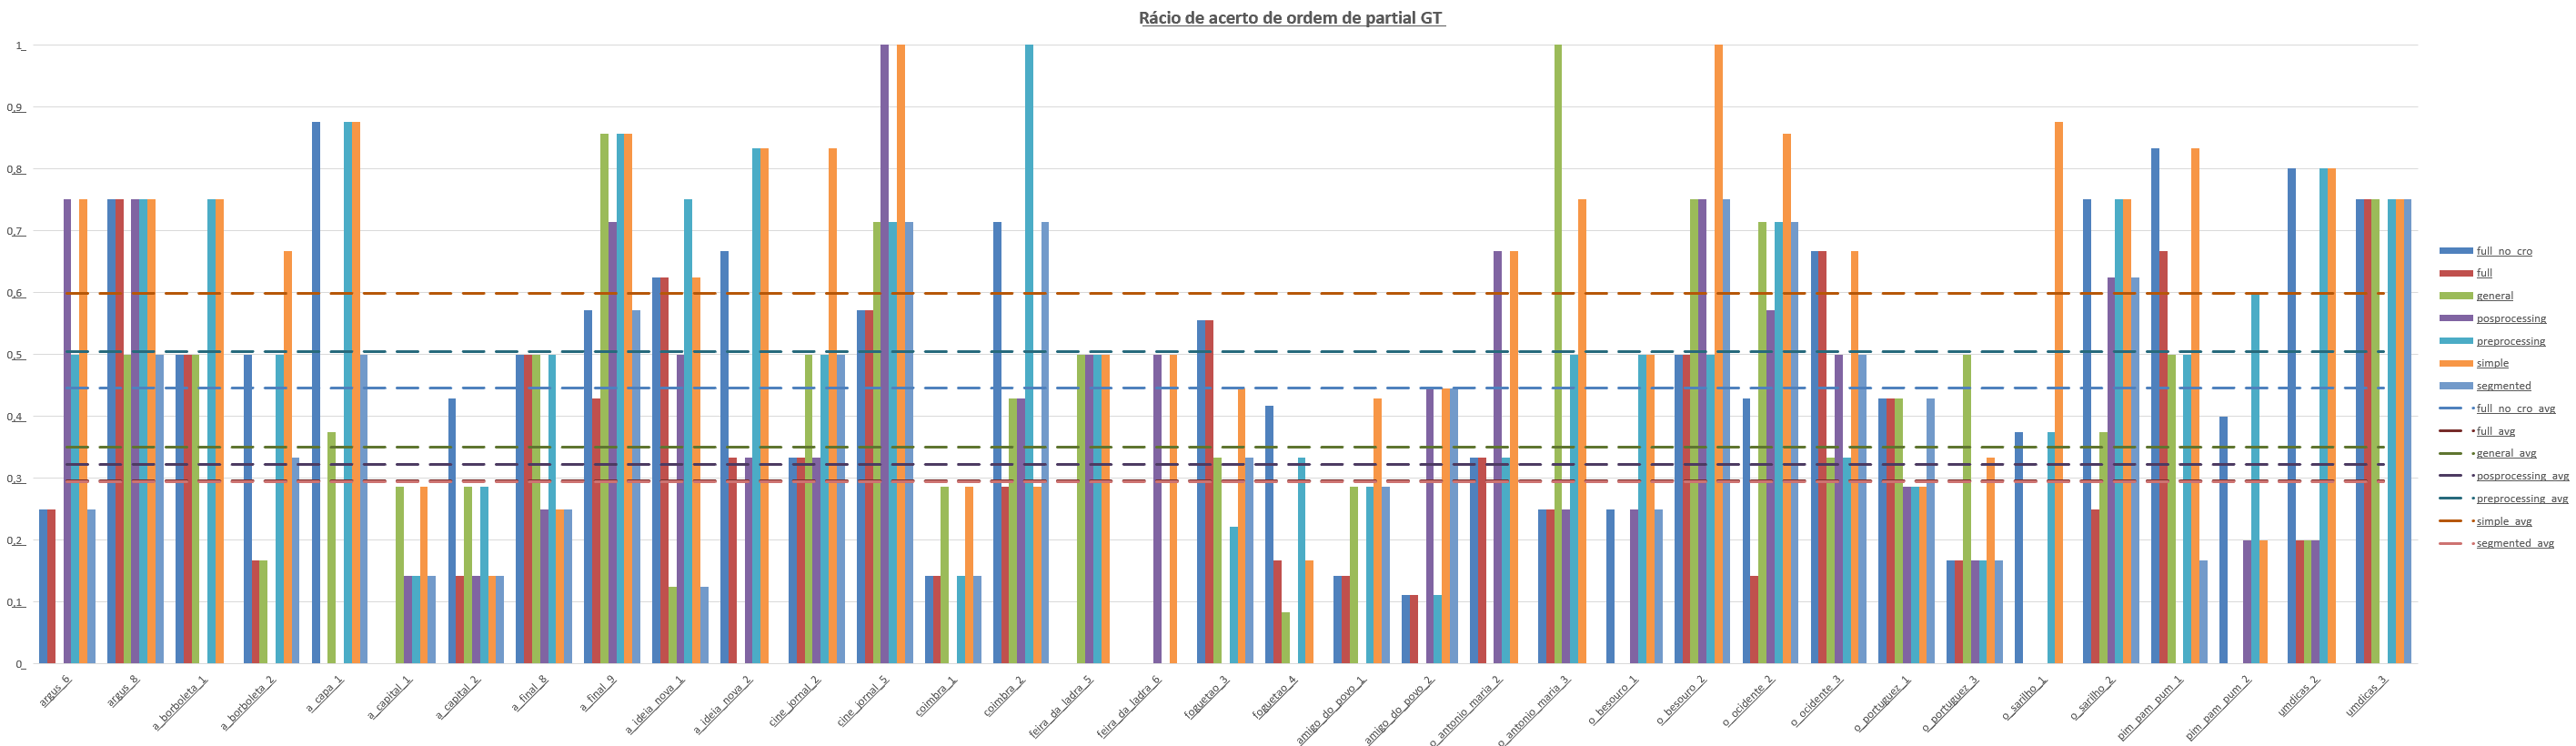
\includegraphics[angle=90,width=0.4\textwidth]{images/resultados/graph_pgt_correct_order_ratio.png}
	\caption{Rácios de acerto da ordem das linhas da Partial GT das diferentes pipelines (alargado).}
	\label{fig:graph_pgt_correct_order_ratio_large}
\end{figure}



\begin{figure}[H]
	\centering
	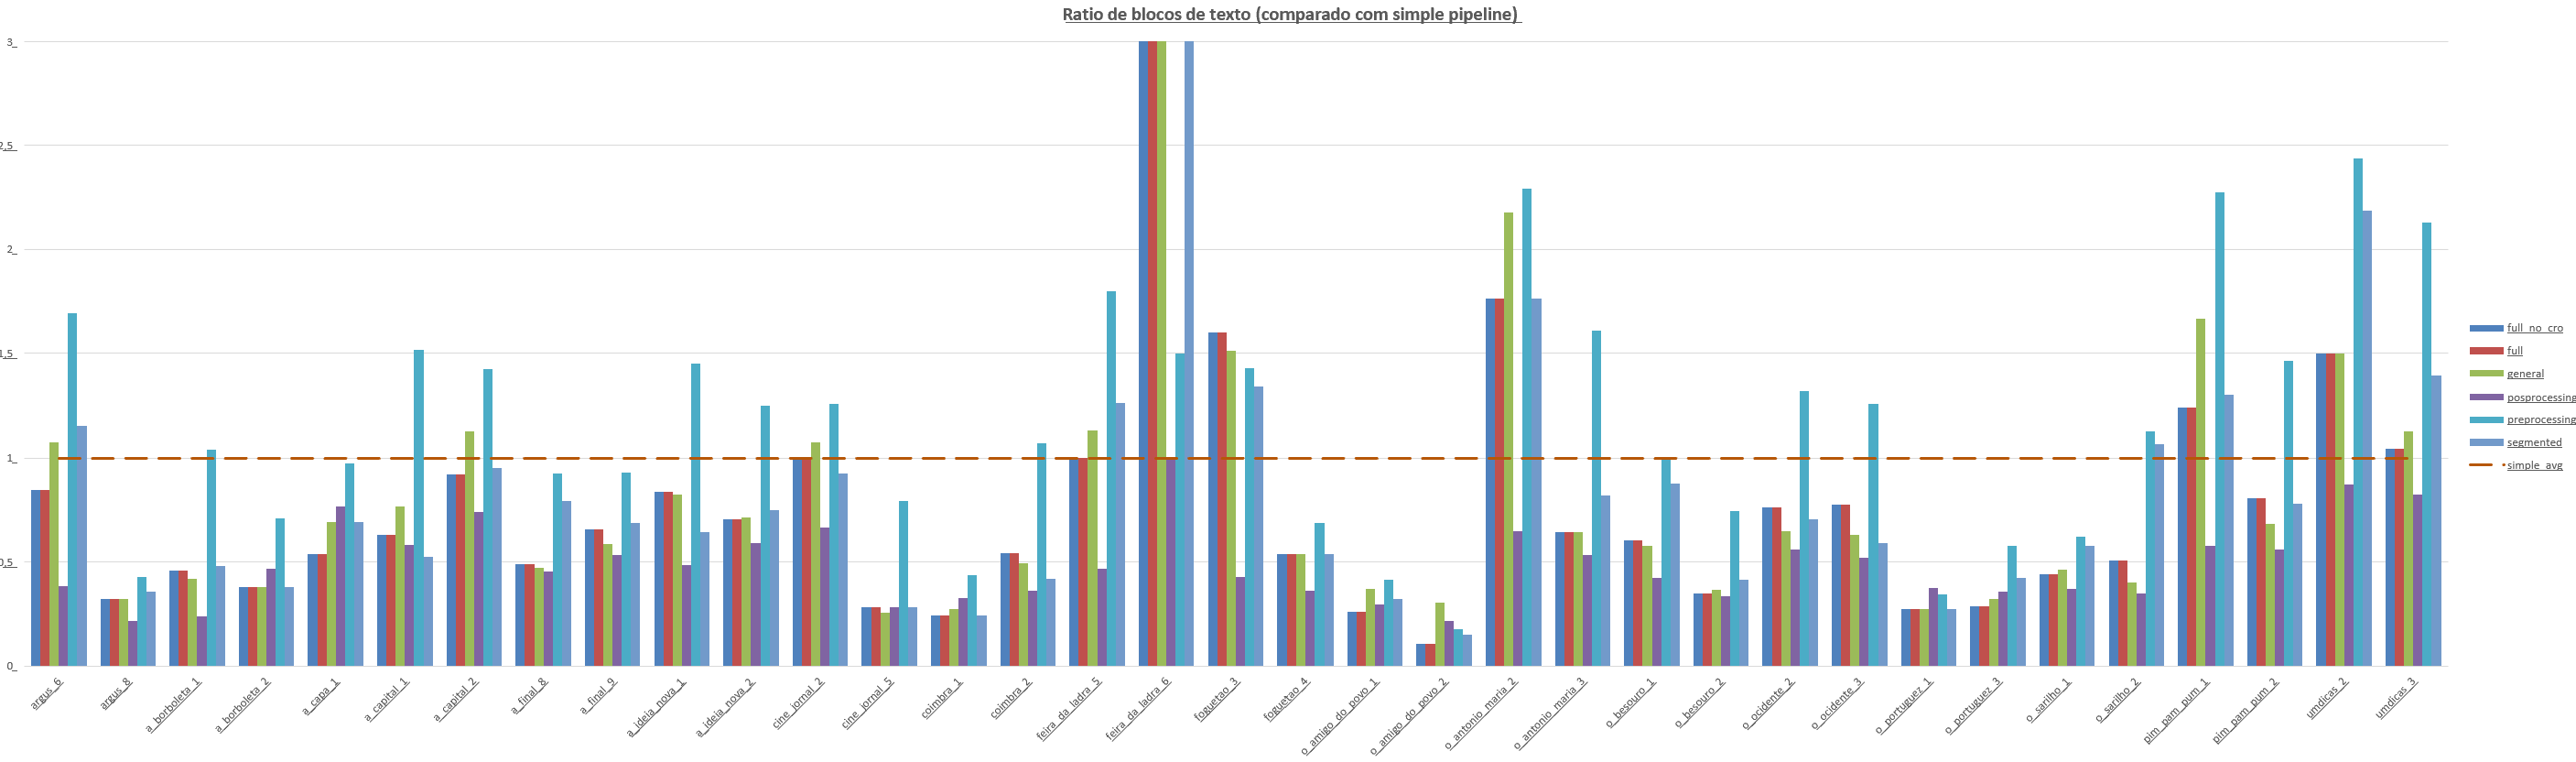
\includegraphics[angle=90,width=0.4\textwidth]{images/resultados/graph_text_block_ratio.png}
	\caption{Rácios de número de blocos de texto relativo à pipeline simples (alargado).}
	\label{fig:graph_text_block_ratio_large}
\end{figure}
